\newenvironment{observationtable}[1][Tabela Obserwacji]{
  \begin{center}
  \renewcommand{\arraystretch}{1.3}
  \textbf{#1}\vspace{0.5em} \\
  \begin{tabular}{|c|c|c|}
  \hline
}{
  \hline
  \end{tabular}
  \end{center}
}

\section{Algorytm \textit{L*}}
\label{sec:l-star}

Algorytm \textit{L*} \cite{L_STAR} wyróżnia się na tle innych algorytmów do odkrywania gramatyki języka regularnego użytych w pracy dzięki swojemu podejściu do uczenia. Większość innych algorytmów opiera się wyłącznie na przykładach pozytywnych lub zarówno na przykładach pozytywnych, jak i negatywnych. Algorytm \textit{L*} wyłamuje się z tej konwencji, wykorzystując zapytania oraz kontrprzykłady do procesu nauki.

Model algorytmu składa się z dwóch aktorów: \textbf{nauczyciela} oraz \textbf{ucznia}. Jego celem jest skonstruowanie minimalnego deterministycznego automatu skończonego (DFA), który rozpoznaje dany język regularny na podstawie ograniczonych interakcji między dwoma uczestnikami procesu.

\subsection{Metoda}

Konstruowanie minimalnego automatu deterministycznego (DFA), który akceptuje język \( L \), odbywa się przy pomocy dwóch rodzajów zapytań:
\begin{itemize}
    \item \textbf{Zapytania o członkostwo (Membership Queries, \textit{MQ}):} Uczeń pyta, czy słowo \( w \) należy do języka \( L \). Nauczyciel odpowiada „tak” (\( w \in L \)) lub „nie” (\( w \notin L \)).
    \item \textbf{Zapytania o równoważność (Equivalence Queries, \textit{EQ}):} Uczeń przedstawia hipotezę \( H \), reprezentującą język \( L(H) \), i pyta, czy \( L(H) = L \). Jeśli hipoteza jest niepoprawna, nauczyciel dostarcza kontrprzykład \( w \), dla którego \( w \in L \) i \( w \notin L(H) \), lub \( w \notin L \) i \( w \in L(H) \).
\end{itemize}

Dla poprawnego działania algorytmu wymagane jest, aby nauczyciel mógł udzielać prawdziwych odpowiedzi na oba rodzaje zadawanych pytań. Nauczyciela często nazywa się również \textbf{wyrocznią}, co jest skrótem myślowym, ponieważ formalnie nauczyciel składa się z pary \textbf{wyroczni (oracles)}: \textit{MQ} i \textit{EQ}. Zazwyczaj to na użytkowniku algorytmu spoczywa odpowiedzialność za określenie nauczyciela, co wymaga już na wstępie posiadania pewnej wiedzy na temat danego języka. Jest to największe ograniczenie w zastosowaniu algorytmu \textit{L*}.

Proces algorytmu \textit{L*} opiera się na iteracyjnym konstruowaniu \textbf{tabeli obserwacji (Observation Table)}, która gromadzi informacje o języku L uzyskane na podstawie zapytań typu \textit{MQ}. Na podstawie zawartości tabeli formułowane są kolejne hipotezy dotyczące automatu DFA, które następnie poddawane są weryfikacji za pomocą zapytań typu \textit{EQ}.

Główne kroki algorytmu:
\begin{enumerate}
    \item \textbf{Inicjalizacja:} Algorytm rozpoczyna od utworzenia tabeli obserwacji wykorzystując minimalne zbiory prefiksów (\( S \)) i sufiksów (\( E \)).
    \item \textbf{Sprawdzanie domknięcia i spójności:} Algorytm weryfikuje, czy tabela obserwacji spełnia wymagania:
    \begin{itemize}
        \item \textbf{Domknięcie:} Każdy prefiks prowadzi do jednego z już znanych stanów.
        \item \textbf{Spójność:} Wiersze tabeli są rozróżnialne za pomocą sufiksów w \( E \).
    \end{itemize}
    Jeśli tabela nie spełnia tych wymagań algorytm zwiększa zbiory \( S \) i \( E \).
    \item \textbf{Tworzenie hipotezy:} Na podstawie tabeli obserwacji generowany jest automat DFA \( H \).
    \item \textbf{Test równoważności:} Hipoteza \( H \) jest testowana za pomocą \textit{EQ}. W przypadku błędu tabela jest aktualizowana na podstawie kontrprzykładu.
    \item \textbf{Terminacja:} Proces kończy się, gdy hipoteza \( H \) jest poprawna.
\end{enumerate}

\subsection{Formalizacja}

Celem tej sekcji jest przedstawienie formalnych podstaw i narzędzi matematycznych, które są niezbędne do zrozumienia algorytmu \( L^* \). W sekcji tej zawarto definicje kluczowych pojęć, takich jak języki regularne i automaty deterministyczne (DFA), które stanowią fundament problemu inferencji języka na podstawie ograniczonego zestawu danych.

\begin{definition}[DFA]  
    Skończony automat deterministyczny (DFA) to piątka uporządkowana \( M = (Q, \Sigma, \delta, q_0, F) \), gdzie:
    \begin{itemize}
        \item \( Q \): skończony zbiór stanów,
        \item \( \Sigma \): alfabet,
        \item \( \delta: Q \times \Sigma \to Q \): funkcja przejścia,
        \item \( q_0 \in Q \): stan początkowy,
        \item \( F \subseteq Q \): zbiór stanów akceptujących.
    \end{itemize}
\end{definition}

\begin{definition}[Akceptowanie słowa]
    Automat \( M \) akceptuje słowo \( w \in \Sigma^* \), jeśli \( \delta(q_0, w) \in F \), gdzie \( \delta(q_0, w) \) oznacza iteracyjne zastosowanie funkcji przejścia \( \delta \) do słowa \( w \).
\end{definition}

\begin{definition}[Język regularny]  
    Język \( L \subseteq \Sigma^* \) zdefiniowany nad alfabetem \( \Sigma \) nazywamy językiem regularnym, jeśli istnieje deterministyczny automat skończony (DFA) \( M = (Q, \Sigma, \delta, q_0, F) \), który akceptuje wszystkie słowa należące do \( L \), i tylko te słowa:
    \[
    L = \{ w \in \Sigma^* \mid M \text{ akceptuje } w \}.
    \]
\end{definition}

Formalizacja DFA pozwala przejść od intuicyjnego opisu języka regularnego do jego precyzyjnej, algebraicznej reprezentacji. Stanowi to punkt wyjścia do rozważania procesu konstrukcji automatu \( H \) na podstawie tabeli obserwacji.

\begin{definition}[Tabela obserwacji] 
    Tabela obserwacji (ObservationTable) to struktura danych definiowana jako trójka \( (S, E, T) \), gdzie:
    \begin{itemize}
        \item \( S \subseteq \Sigma^* \): skończony zbiór prefiksów,
        \item \( E \subseteq \Sigma^* \): skończony zbiór sufiksów,
        \item \( T: (S \cup S \cdot \Sigma) \times E \to \{0, 1\} \): funkcja wartościująca wynik zapytania \( MQ(s \cdot e) \), gdzie \( s \in S \cup S \cdot \Sigma \) i \( e \in E \).
    \end{itemize}
\end{definition}

Tabela obserwacji jest kluczowym elementem algorytmu \( L^* \). Przechowuje informacje o zachowaniu języka \( L \) względem słów w zbiorach \( S \) i \( E \). Dzięki temu pozwala grupować słowa w klasy równoważności, co jest podstawą do wyznaczenia stanów DFA.

\begin{definition}[Domknięcie] 
    Tabela obserwacji jest domknięta jeśli dla każdego \( s \in S \cdot \Sigma \), istnieje \( s' \in S \), taki że \( \forall e \in E, \, T(s, e) = T(s', e) \).
\end{definition}
\begin{definition}[Spójność]
    Tabela obserwacji jest spójna, jeśli dla dowolnych \( s_1, s_2 \in S \), spełniających warunek:
    \[
    \forall e \in E, \, T(s_1, e) = T(s_2, e),
    \]
    zachodzi również:
    \[
    \forall a \in \Sigma, \, \forall e \in E, \, T(s_1 \cdot a, e) = T(s_2 \cdot a, e).
    \]
\end{definition}

Warunki te zapewniają, że tabela obserwacji reprezentuje wystarczająco bogatą informację o języku \( L \), aby można było skonstruować poprawny DFA. \textbf{Domknięcie} gwarantuje, że wszystkie przejścia są uwzględnione w zbiorze \( S \), natomiast \textbf{spójność} zapewnia, że tabela jest zgodna z oczekiwanym zachowaniem języka.

\begin{definition}[Tworzenie hipotezy]
    Na podstawie tabeli (ObservationTable), która spełnia warunki \textbf{domknięcia} i \textbf{spójności}, można skonstruować DFA \( H = (Q, \Sigma, \delta, q_0, F) \), gdzie:
    \begin{itemize}
        \item \( Q = \{[s] \mid s \in S\} \), gdzie \( [s] \) oznacza klasę równoważności \( s \) w \( T \),
        \item \( \delta([s], a) = [s \cdot a] \),
        \item \( q_0 = [\epsilon] \),
        \item \( F = \{[s] \mid T(s, \epsilon) = 1\} \).
    \end{itemize}
\end{definition}

Klasy równoważności w \( T \) grupują słowa \( s \in S \) o identycznym zachowaniu względem języka \( L \). Dzięki temu DFA \( H \) przechodzi między stanami odpowiadającymi tym klasom, w oparciu o funkcję przejścia \( \delta \).

\begin{definition}[Kontrprzykład]
    Kontrprzykład dla hipotezy H odnośnie języka L nazywamy takie $w$, że \( w \in L \setminus L(H) \cup L(H) \setminus L \).
\end{definition}

\begin{definition}[Zapytanie o członkostwo]
    \emph{Zapytanie o członkostwo} (\emph{Membership Query}) to funkcja \( MQ: \Sigma^* \to \{0, 1\} \), która dla danego słowa \( w \in \Sigma^* \) zwraca \( 1 \), jeśli \( w \in L \), lub \( 0 \) w przeciwnym przypadku.
\end{definition}

\begin{definition}[Zapytanie o równoważność]
    \emph{Zapytanie o równoważność} (\emph{Equivalence Query}) to funkcja \( EQ: \mathcal{H} \to (\Sigma^* \cup \{\text{brak}\}) \), która dla hipotezy \( H \) zwraca:
    \begin{itemize}
        \item brak, jeśli \( L(H) = L \), czyli hipoteza \( H \) jest równoważna językowi \( L \).
        \item w przeciwnym wypadku \textbf{kontrprzykład},
    \end{itemize}
\end{definition}


Jeśli język generowany z hipotezy \( H \) nie jest równoważny \( L \), Nauczyciel dostarcza kontrprzykład \( w \). Prefiksy \( w \) są dodawane do \( S \), a tabela jest aktualizowana zgodnie z wynikami zapytań \( MQ \). Proces ten jest iteracyjny i pozwala na sukcesywne udoskonalanie tabeli obserwacji oraz hipotezy automatu \( H \), aż do uzyskania poprawnego modelu języka.

\subsection{Złożoność}

Algorytm \textit{L*} składa się z kilku etapów, których złożoność można szczegółowo przeanalizować. Złożoność czasowa algorytmu jest wielomianowa, co zostało udowodnione \cite{L_STAR}. Aby wyliczyć złożoność pamięciową trzeba zdefiniować:
\begin{itemize}
    \item \(n\) - liczba stanów szukanego minimalnego DFA,
    \item \(m\) - maksymalna długość kontrprzykładu,
    \item \(|\Sigma|\) - rozmiar alfabetu.
\end{itemize}

Struktura danych w algorytmie składa się z dwóch komponentów:
\begin{itemize}
    \item \textbf{Tabela obserwacji:}
    \begin{itemize}
        \item Zbiór \(S\) (prefiksy): maksymalnie \(O(n + m \cdot (n - 1))\) wpisów,
        \item Zbiór \(E\) (sufiksy): maksymalnie \(O(n)\) wpisów,
        \item Całkowity rozmiar tabeli: \(O(n \cdot m)\).
    \end{itemize}
    \item \textbf{DFA hipotezy:} DFA może mieć maksymalnie \(n\) stanów i \(O(n \cdot |\Sigma|)\) przejść.
\end{itemize}

Algorytm wymaga pamięci na tabelę obserwacji oraz strukturę DFA, stąd można obliczyć łączną złożoność pamięciową:
\[
O(n \cdot m + n \cdot |\Sigma|).
\]

Podsumowując czynnikami wpływającymi na złożoność pamięciową są:
\begin{itemize}
    \item \textbf{Rozmiar alfabetu (\(|\Sigma|\))}: Większy alfabet oznacza więcej przejść w tabeli obserwacji i DFA.
    \item \textbf{Długość kontrprzykładów (\(m\))}: Dłuższe kontrprzykłady zwiększają liczbę zapytań o członkostwo i rozmiar tabeli obserwacji.
    \item \textbf{Liczba stanów DFA (\(n\))}: Więcej stanów oznacza większą tabelę obserwacji i więcej iteracji algorytmu.
\end{itemize}

\subsection{Przykłady działania}

Aby rozjaśnić działanie algorytmu \textit{L*}, rozważmy proste języki $L_1$ i $L_2$

\[
L_1 = \{ w \in \{a, b\}^* \mid \text{liczba liter } a \text{ w } w \text{ jest parzysta} \}.
\]
\[
L_2 = \{ w \in \{a, b\}^* \mid \text{liczba liter } a \text{ jest parzysta lub liczba liter } b \text{ jest parzysta} \}.
\]

Minimalny DFA dla języka $L_1$ ma dwa stany:
\begin{itemize}
    \item Stan $s_0$: parzysta liczba $a$,
    \item Stan $s_1$: nieparzysta liczba $a$.
\end{itemize}

Dla języka $L_2$ zawiera cztery stany, ponieważ istnieją cztery możliwe kombinacje parzystości:
\begin{itemize}
    \item Stan $s_0$: parzysta liczba $a$ i parzysta liczba $b$,
    \item Stan $s_1$: nieparzysta liczba $a$ i parzysta liczba $b$,
    \item Stan $s_2$: nieparzysta liczba $a$ i nieparzysta liczba $b$,
    \item Stan $s_3$: parzysta liczba $a$ i nieparzysta liczba $b$.
\end{itemize}

Schematy minimalnych DFA można zobaczyć kolejno na rysunkach \ref{fig:dfa_even_a} i \ref{fig:dfa_even_a_or_even_b}.

\subsubsection{Przykład 1}

\paragraph*{Inicjalizacja tabeli obserwacji.}
Rozpoczynamy od tworzenia minimalnych zbiorów \textit{S} i \textit{E}:
\[
S = \{\epsilon\}, \quad E = \{\epsilon\}.
\]
Uczeń zadaje pytanie o członkostwo \( MQ(\epsilon) \), a Nauczyciel odpowiada „tak”, ponieważ \( \epsilon \in L \). Na tej podstawie konstruujemy tabelę \ref{tab:lang_1_observation_1}.

\begin{table}
    \centering
    \begin{tabular}{c|c}
        \diagbox{\( S \cup (S \cdot \Sigma) \)}{$E$} & \( \epsilon \) \\
        \hline
        $\epsilon$ & 1 \\
    \end{tabular}
    \caption{Tabela obserwacji $T_0$ dla języka \( L_1 \).}
    \label{tab:lang_1_observation_1}
\end{table}

\paragraph*{Dodanie nowych wierszy.}
Uczeń dodaje \( S \cdot \Sigma = \{a, b\} \) do tabeli i zadaje zapytania o członkostwo:
\[
MQ(a) = 0, \quad MQ(b) = 1.
\]
Zaktualizowaną tabelę widać w tabeli \ref{tab:lang_1_observation_2}.Tabela jest \textbf{niedomknięta}, ponieważ dla \(a\) nie istnieje takie \(s \in S \), że \( \forall e \in E, \, T(a, e) = T(s, e) \).

\begin{table}
    \centering
    \begin{tabular}{c|c}
        \diagbox{\( S \cup (S \cdot \Sigma) \)}{$E$} & \( \epsilon \) \\
        \hline
        $\epsilon$ & 1 \\
        \hline
        $a$              & 0 \\
        $b$              & 1 \\
    \end{tabular}
    \caption{Tabela obserwacji $T_1$ dla języka \( L_1 \).}
    \label{tab:lang_1_observation_2}
\end{table}

\paragraph*{Rozszerzenie \( S \).}
Dodajemy \( a \) do \( S \), aby tabela była domknięta:
\[
S = \{\epsilon, a\}.
\]
Uczeń zadaje zapytania dla nowych rozszerzeń \( S \cdot \Sigma \):
\[
MQ(aa) = 1, \quad MQ(ab) = 0.
\]
Nowe obserwacje widać w tabeli \ref{tab:lang_1_observation_3}. Tabela jest teraz \textbf{domknięta}. Jest też ona \textbf{spójna}. Możemy teraz skonstruować hipotezę.

\begin{table}
    \centering
    \begin{tabular}{c|c}
        \diagbox{\( S \cup (S \cdot \Sigma) \)}{$E$} & \( \epsilon \) \\
        \hline
        $\epsilon$      & 1 \\
        $a$             & 0 \\
        \hline
        $b$             & 1 \\
        $aa$            & 1 \\
        $ab$            & 0 \\
    \end{tabular}
    \caption{Tabela obserwacji $T_2$ dla języka \( L_1 \).}
    \label{tab:lang_1_observation_3}
\end{table}

\paragraph*{Konstrukcja hipotezy.}
Na podstawie tabeli obserwacji \ref{tab:lang_1_observation_3} konstruujemy hipotezę automatu DFA:
\begin{itemize}
    \item \textbf{Stany DFA:} \( q_\epsilon, q_a \), odpowiadające \( T(\epsilon, \epsilon) \) oraz \( T(a, \epsilon) \).
    \item \textbf{Przejścia:}
    \begin{align*}
        & q_\epsilon \xrightarrow{a} q_a, \quad q_\epsilon \xrightarrow{b} q_\epsilon, \\
        & q_a \xrightarrow{a} q_\epsilon, \quad q_a \xrightarrow{b} q_a.
    \end{align*}
    \item \textbf{Stan początkowy:} \( q_\epsilon \), ponieważ odpowiada wierszowi \( \epsilon \).
    \item \textbf{Stany akceptujące:} \( q_\epsilon \), ponieważ odpowiada \( T(\epsilon, \epsilon) = 1 \).
    \item \textbf{Stany nieakceptujące:} \( q_a \), ponieważ \( T(a, \epsilon) = 0 \).
\end{itemize}

\paragraph*{Testowanie hipotezy.}
Hipoteza jest testowana przez zapytanie o równoważność (EQ). Nauczyciel odpowiada "tak" co kończy działanie algorytmu. 

\paragraph*{Ostateczny automat.}
Automat DFA reprezentujący język o parzystej liczbie \( a \):
\[
\begin{array}{c|c|c}
\text{Stan} & a & b \\
\hline
\rightarrow * q_\epsilon & q_a & q_\epsilon \\
q_a & q_\epsilon & q_a \\
\end{array}
\]

\begin{figure}[ht]
    \centering
    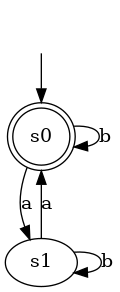
\includegraphics[width=0.2\linewidth]{images/dfa_even_a.png}
    \caption{Minimalny DFA generujący język $L_1$.}
    \label{fig:dfa_even_a}
\end{figure}

\subsubsection{Przykład 2}

\paragraph*{Dodanie nowych wierszy.}
Inicjalizacja tabeli obserwacji przebiega tak samo jak w przykładzie pierwszym.
Uczeń rozszerza \( S \) o \( S \cdot \Sigma = \{a, b\} \) i zadaje pytania:
\[
MQ(a) = 0, \quad MQ(b) = 0.
\]
Tabelę po aktualizacji widać w tabeli \ref{tab:lang_2_observation_1}. Jest ona \textbf{spójna} i \textbf{domknięta}. Można, więc skonstruować hipotezę.

\begin{table}
    \centering
    \begin{tabular}{c|c}
        \diagbox{\( S \cup (S \cdot \Sigma) \)}{$E$} & \( \epsilon \) \\
        \hline
        $\epsilon$      & 1 \\
        \hline
        $a$             & 1 \\
        $b$             & 1 \\
    \end{tabular}
    \caption{Tabela obserwacji $T_1$ dla języka \( L_2 \).}
    \label{tab:lang_2_observation_1}
\end{table}

\paragraph*{Konstrukcja hipotezy $H_1$.}
Na podstawie tabeli obserwacji \ref{tab:lang_2_observation_1} konstruujemy hipotezę:
\begin{itemize}
    \item \textbf{Stany DFA:} \( q_\epsilon \), odpowiadający unikalnym wierszom tabeli.
    \item \textbf{Przejścia:}
    \begin{align*}
        & q_\epsilon \xrightarrow{a} q_\epsilon, \quad q_\epsilon \xrightarrow{b} q_\epsilon.
    \end{align*}
    \item \textbf{Stan początkowy:} \( q_\epsilon \).
    \item \textbf{Stany akceptujące:} \( q_\epsilon \).
\end{itemize}

\paragraph*{Testowanie hipotezy $H_1$.}
Hipoteza jest testowana przez zapytanie o równoważność (EQ). Można wybrać nieskończenie wiele kontrprzykładów, ale ja przyjmę, że nauczyciel zwraca $ba$.

\paragraph*{Aktualizacja tabeli obserwacji.}
Po otrzymaniu kontrprzykładu \( ba \), algorytm aktualizuje tabelę obserwacji. Wszystkie prefiksy \( ba \) są dodawane do zbioru \( S \), co prowadzi do:
\[
S = \{\epsilon, b, ba\}.
\]
Uczeń zadaje zapytania \( MQ \) dla nowych elementów \( S \cup (S \cdot \Sigma) \). Wyniki zapytań są następujące:
\[
MQ(ba) = 0, \quad MQ(baa) = 1, \quad MQ(bab) = 1.
\]
Na tej podstawie aktualizujemy tabelę obserwacji. Wynikową tabelę obserwacji pokazano w tabeli \ref{tab:lang_2_observation_2}. Jest ona \textbf{domknięta} i \textbf{niespójna}, ponieważ \( T(\epsilon, \epsilon) = T(b, \epsilon) \), a \( T(\epsilon \cdot a, \epsilon) \neq T(b \cdot a, \epsilon) \), stąd $a$ jest rozróżniającym sufiksem. Dodajemy $a$ do $E$ i uzupełniamy tabelę obserwacji \ref{tab:lang_2_observation_3}. Jest ona \textbf{domknięta} i \textbf{spójna}, więc możemy skonstruować hipotezę.
\[
MQ(\epsilon \cdot a) = 1, \quad MQ(b \cdot a) = 0, \quad MQ(ba \cdot a) = 1,
\]
\[
MQ(a \cdot a) = 1, \quad MQ(bb \cdot a) = 1, \quad MQ(baa \cdot a) = 0, \quad MQ(bab \cdot a) = 1.
\]

\begin{table}
    \centering
    \begin{tabular}{c|c}
        \diagbox{\( S \cup (S \cdot \Sigma) \)}{$E$} & \( \epsilon \) \\
        \hline
        $\epsilon$      & 1 \\
        $b$             & 1 \\
        $ba$            & 0 \\
        \hline
        $a$             & 1 \\
        $bb$            & 1 \\
        $baa$           & 1 \\
        $bab$           & 1 \\
    \end{tabular}
    \caption{Tabela obserwacji $T_2$ dla języka \( L_2 \).}
    \label{tab:lang_2_observation_2}
\end{table}

\begin{table}
    \centering
    \begin{tabular}{c|c|c}
        \diagbox{\( S \cup (S \cdot \Sigma) \)}{$E$} & \( \epsilon \) & $a$ \\
        \hline
        $\epsilon$      & 1 & 1 \\
        $b$             & 1 & 0 \\
        $ba$            & 0 & 1 \\
        \hline
        $a$             & 1 & 1 \\
        $bb$            & 1 & 1 \\
        $baa$           & 1 & 0 \\
        $bab$           & 1 & 1 \\
    \end{tabular}
    \caption{Tabela obserwacji $T_3$ dla języka \( L_2 \).}
    \label{tab:lang_2_observation_3}
\end{table}

\paragraph*{Konstrukcja hipotezy $H_2$.}
Na podstawie tabeli obserwacji \ref{tab:lang_2_observation_3} konstruujemy hipotezę:
\begin{itemize}
    \item \textbf{Stany DFA:} \( q_\epsilon, q_b, q_{ba} \), odpowiadający unikalnym wierszom tabeli.
    \item \textbf{Przejścia:}
    \begin{align*}
        & q_\epsilon \xrightarrow{a} q_\epsilon, \quad q_\epsilon \xrightarrow{b} q_b, \\
        & q_b \xrightarrow{a} q_{ba}, \quad q_b \xrightarrow{b} q_\epsilon, \\
        & q_{ba} \xrightarrow{a} q_\epsilon, \quad q_{ba} \xrightarrow{b} q_b.
    \end{align*}
    \item \textbf{Stan początkowy:} \( q_\epsilon \).
    \item \textbf{Stany akceptujące:} \( q_\epsilon, q_b \).
\end{itemize}

\paragraph*{Testowanie hipotezy $H_2$.}
Hipoteza jest testowana przez zapytanie o równoważność (EQ). Można wybrać nieskończenie wiele kontrprzykładów, ale ja przyjmę, że nauczyciel zwraca $ab$. Jest to kontrprzykład, ponieważ \( ab \in L(H) \land ab \notin L \). 

\paragraph*{Aktualizacja tabeli obserwacji.}
Po otrzymaniu kontrprzykładu \( ab \), algorytm aktualizuje tabelę obserwacji. Na początek dodajemy \( a \) oraz \( ab \) do zbioru \( S \), co prowadzi do:
\[
S = \{ \epsilon, a, b, ab, ba \}.
\]
Uczeń zadaje pytania \( MQ \) dla nowych elementów \( S \cup (S \cdot \Sigma) \). Wyniki zapytań są następujące:
\[
MQ(aa) = 1, \quad MQ(ab) = 0, \quad MQ(aba) = 1, \quad MQ(abb) = 1,
\]
\[
MQ(aa \cdot a) = 1, \quad MQ(ab \cdot a) = 1, \quad MQ(aba \cdot a) = 0, \quad MQ(abb \cdot a) = 1.
\]
Na tej podstawie aktualizujemy tabelę obserwacji. Wynikową tabelę obserwacji pokazano w tabeli \ref{tab:lang_2_observation_4}. Tabela \( T_4 \) jest \textbf{domknięta}, ale \textbf{niespójna}, ponieważ wiersz dla $\epsilon$ jest taki sam jak wiersz dla $a$, a wiersz dla \( \epsilon \cdot b \) jest inny niż wiersz dla \( a \cdot b \), stąd $b$ jest rozróżniającym sufiksem. Dodajemy $b$ do $E$ i uzupełniamy tabelę obserwacji \ref{tab:lang_2_observation_5}. 
Dodanie \( b \) do \( E \) pozwala naprawić niespójność, rozróżniając zachowanie stanów dla różnych sufiksów. Uczeń zadaje nowe zapytania \( MQ \) dla wszystkich \( S \cup (S \cdot \Sigma) \) i uzupełnia tabelę. Wyniki zapytań:
\[
MQ(\epsilon \cdot b) = 1, \quad MQ(a \cdot b) = 0, \quad MQ(b \cdot b) = 1, \quad MQ(ab \cdot b) = 1.
\]
Jest ona \textbf{domknięta} i \textbf{spójna}. 

\begin{table}
    \centering
    \begin{tabular}{c|c|c}
        \diagbox{\( S \cup (S \cdot \Sigma) \)}{$E$} & \( \epsilon \) & $a$ \\
        \hline
        $\epsilon$      & 1 & 1 \\
        $a$             & 1 & 1 \\
        $ab$            & 0 & 1 \\
        $b$             & 1 & 0 \\
        $ba$            & 0 & 1 \\
        \hline
        $aa$            & 1 & 1 \\
        $bb$            & 1 & 1 \\
        $aba$           & 1 & 0 \\
        $abb$           & 1 & 1 \\
        $baa$           & 1 & 0 \\
        $bab$           & 1 & 1 \\
    \end{tabular}
    \caption{Tabela obserwacji $T_4$ dla języka \( L_2 \) po dodaniu \( a \) i \( ab \) do \( S \).}
    \label{tab:lang_2_observation_4}
\end{table}

\begin{table}
    \centering
    \begin{tabular}{c|c|c|c}
        \diagbox{\( S \cup (S \cdot \Sigma) \)}{$E$} & $\epsilon$ & $a$ & $b$ \\
        \hline
        $\epsilon$      & 1 & 1 & 1 \\
        $a$             & 1 & 1 & 0 \\
        $ab$            & 0 & 1 & 1 \\
        $b$             & 1 & 0 & 1 \\
        $ba$            & 0 & 1 & 1 \\
        \hline
        $aa$            & 1 & 1 & 1 \\
        $bb$            & 1 & 1 & 1 \\
        $aba$           & 1 & 0 & 1 \\
        $abb$           & 1 & 1 & 0 \\
        $baa$           & 1 & 0 & 1 \\
        $bab$           & 1 & 1 & 0 \\
    \end{tabular}
    \caption{Tabela obserwacji $T_5$ dla języka \( L_2 \) po dodaniu \( b \) do \( E \).}
    \label{tab:lang_2_observation_5}
\end{table}

\paragraph*{Konstrukcja hipotezy $H_3$.}
Na podstawie tabeli obserwacji konstruujemy hipotezę DFA:
\begin{itemize}
    \item \textbf{Stany DFA:} \( q_\epsilon, q_a, q_b, q_{ab} \)
    \item \textbf{Przejścia:}
    \begin{align*}
        & q_\epsilon \xrightarrow{a} q_a, \quad q_\epsilon \xrightarrow{b} q_b, \\
        & q_a \xrightarrow{a} q_\epsilon, \quad q_a \xrightarrow{b} q_{ab}, \\
        & q_b \xrightarrow{a} q_{ab}, \quad q_b \xrightarrow{b} q_\epsilon, \\
        & q_{ab} \xrightarrow{a} q_b, \quad q_{ab} \xrightarrow{b} q_a.
    \end{align*}
    \item \textbf{Stan początkowy:} \( q_\epsilon \).
    \item \textbf{Stany akceptujące:} \( q_\epsilon, q_a, q_b \)
\end{itemize}

\paragraph*{Testowanie hipotezy $H_3$.}
Hipoteza jest testowana przez zapytanie o równoważność (EQ). Nauczyciel odpowiada "tak", co kończy działanie algorytmu.

\paragraph*{Ostateczny automat.}
Automat DFA reprezentujący język \( L \) ma następującą macierz przejść:
\[
\begin{array}{c|c|c}
\text{Stan} & a & b \\
\hline
\rightarrow * q_\epsilon & q_a & q_b \\
* q_a & q_\epsilon & q_{ab} \\
* q_b & q_{ab} & q_\epsilon \\
q_{ab} & q_b & q_a \\
\end{array}
\]

\begin{figure}[ht]
    \centering
    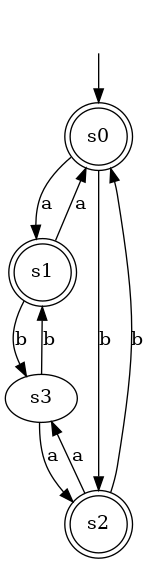
\includegraphics[width=0.2\linewidth]{images/dfa_even_a_or_even_b.png}
    \caption{Minimalny DFA dla języka \( L_2 \): parzystość \( a \) lub \( b \).}
    \label{fig:dfa_even_a_or_even_b}
\end{figure}

% Opcjonalnie zastosowania i rozszerzenia
